% Load tex files defining the some graphics.

In the \secref{valid_priors}, we proved that directional derivatives exist for
$p \in [1, \infty)$, at least for all perturbations of the form given by
\defref{prior_nl_pert}. However, when using a linear approximation to searching
over a in infinite dimensional space, one needs to ask not only whether the
derivative exists, but also whether the derivative forms a uniformly good
approximation to the original function for every $\phi \in \ball_p(\delta)$. In
functionaly analysis, one way to characterize the uniform accuracy of the
derivative is through the concept of Fr{\'e}chet, or bounded, differentiability.

%%%%%%%%%%%%%%%%%%%%%%%%%%%%%%%%%%%%%%%%%%%%%%%%%%%%%%%%%%%%%%%%%%%%%%%%%%%
%%%%%%%%%%%%%%%%%%%%%%%%%%%%%%%%%%%%%%%%%%%%%%%%%%%%%%%%%%%%%%%%%%%%%%%%%%%
\begin{defn}\deflabel{diffable_classes}
    (\citep[Definition 4.5]{zeidler:2013:functional})
%
Let $B_1$ and $B_2$ denote Banach spaces, and let $\ball_1 \subseteq B_1$ define
an open neighborhood of $\phi_0 \in B_1$.  Fix a function $f: \ball_1
\mapsto B_2$.

The function $f$ is {\em directionally differentiable} (also known as a Gateaux
differentiable) if there exists a bounded linear functional $f^{\mathrm{lin}}:
B_1 \mapsto B_2$ such that the following condition holds for any
$\phi$ with $\norm{\phi - \phi_0} < \infty$:
%
\begin{align*}
%
%\textrm{For any }\phi\textrm{ with }\norm{\phi - \phi_0} < \infty\textrm{, }
\lim_{t \rightarrow 0}
    \frac{f(\phi) - f(\phi_0) -
          f^{\mathrm{lin}}(t (\phi - \phi_0) )
         }{t} \rightarrow 0.
%
\end{align*}
%

Similarly, the function $f$ is {\em boundedly differentiable} (also known as
Fr{\'echet} differentiable) at $\phi_0$ if we can take the limit uniformly in
$\phi$:
%
\begin{align*}
%
\lim_{t \rightarrow 0}
    \sup_{\phi: \norm{\phi - \phi_0} = 1}
    \frac{f(\phi) - f(\phi_0) -
          f^{\mathrm{lin}}(t (\phi - \phi_0))
         }{t} \rightarrow 0.
%
\end{align*}
%
\end{defn}
%%%%%%%%%%%%%%%%%%%%%%%%%%%%%%%%%%%%%%%%%%%%%%%%%%%%%%%%%%%%%%%%%%%%%%%%%%%

Note that we used the same notation $f^{\mathrm{lin}}$ for both derivatives in
\defref{diffable_classes}.  In fact, if a function is Fr{\'e}chet differentiable
then the two derivatives must coincide \citep[Proposition
4.8]{zeidler:2013:functional}, which justifies our notation.

Before proceeding with the more complicated discussion of $p \in [1, \infty)$,
we observe that the stringent requirements of the $\lp{\mu,\infty}$ ball
are sufficient to guarantee Fr{\'e}chet differentiability.

%%%%%%%%%%%%%%%%%%%%%%%%%%%%%%%%%%%%%%%%%%%%%%%%%%%%%%%%%%%%%%%%%%%%%%%%%%%%
%%%%%%%%%%%%%%%%%%%%%%%%%%%%%%%%%%%%%%%%%%%%%%%%%%%%%%%%%%%%%%%%%%%%%%%%%%%%
\begin{assu}\assulabel{q_fun_stick_regular}
%
Assume that the variational approximations $\q(\nu \vert \etanuk)$ to the
stick-breaking posteriors satisfy \assuref{dist_fun_nice} with $\eta_0 =
\etaopt$ and with $\psi(\zeta, \t) = 1$.
%
\end{assu}
%%%%%%%%%%%%%%%%%%%%%%%%%%%%%%%%%%%%%%%%%%%%%%%%%%%%%%%%%%%%%%%%%%%%%%%%%%%%


%%%%%%%%%%%%%%%%%%%%%%%%%%%%%%%%%%%%%%%%%%%%%%%%%%%%%%%%%%%%%%%%%%%%%%%%%%%%
%%%%%%%%%%%%%%%%%%%%%%%%%%%%%%%%%%%%%%%%%%%%%%%%%%%%%%%%%%%%%%%%%%%%%%%%%%%%
\begin{thm}\thmlabel{eta_phi_deriv}
%
Let \assuref{kl_opt_ok, q_fun_stick_regular} hold. Then the map $\phi \mapsto
\etaopt(\phi)$ is well-defined and continuously Fr{\'e}chet differentiable in a
neighborhood of $\phiz$ as a map from $\lp{\mu,\infty}$ to $\mathbb{R}^\etadim$,
with the derivative given in \corref{etafun_deriv_form}.

(For a proof, see \appref{proofs} \proofref{eta_phi_deriv}.)

\end{thm}
%%%%%%%%%%%%%%%%%%%%%%%%%%%%%%%%%%%%%%%%%%%%%%%%%%%%%%%%%%%%%%%%%%%%%%%%%%%%

As observed in \thmref{pert_well_defined} and \exref{beta_inf_norm}, the
$\ball_{\mu,\infty}(\delta)$ is a restrictive set.  No matter how large
$\delta$ is, there exist valid priors outside of $\ball_{\mu,\infty}(\delta)$.
\Thmref{eta_phi_deriv} rewards this restrictiveness with differentiability---at
the expense of considering a limited set of priors, we are guaranteed that
the derivatives satisfy the minimal requirements in a ball around $\phiz$.

We now turn to the more expressive unit ball with $p \in [1, \infty)$. Note that
\thmref{lp_derivative} and \corref{pertset_bounded_below} above proved that {\em
directional derivatives} exits for all $\phi \in \pertset$ when $p \in [1,
\infty)$.  We also showed in \thmref{pert_well_defined} and \exref{lp_negative}
that $\KL{\eta, \phi}$ cannot be defined, at least not naiveley, for all $\phi
\in \ball_{\mu,p}(\delta)$, no matter how small $\delta$. Since, in a sense, we
are only interested in $\phi \in \pertset$, we might as whether we cannot form
some smooth, Fr{\'e}chet differentiable extension of the KL divergence to $\phi$
outside $\pertset$, e.g. of the form
%
\begin{align*}
%
\KLhat{\eta, \phi} :=
\begin{cases}
    \KL{\eta, \phi} & \textrm{when }\essinf_{\theta \sim \mu}
        \frac{\phi(\theta)}{\pbase(\theta)^{1/p}} > -\infty\\
    \KL{\eta, \phiz} & \textrm{otherwise}.
\end{cases}
%
\end{align*}
%
Our key result below is be that no such extension will be Fr{\'e}chet
differentiable.

In order to motivate our concern about differentiability, it will be useful to
consider the following example in $\mathbb{R}^2$ of a function that is
directionally differentiable but not Fr{\'e}chet differentiable.

%%%%%%%%%%%%%%%%%%%%%%%%%%%%%%%%%%%%%%%%%%%%%%%%%%%%%%%%%%%%%%%%%%%%%%%%%
%%%%%%%%%%%%%%%%%%%%%%%%%%%%%%%%%%%%%%%%%%%%%%%%%%%%%%%%%%%%%%%%%%%%%%%%%
\begin{ex}\exlabel{r2_pathological}
%
Consider $(x_1, x_2) \in \mathbb{R}^2$ and the polar coordinates $r :=
\sqrt{x_1^2 + x_2^2}$ and $\theta := \arctan(x_2 / x_1)$.  Let $\{\pi k: k \in
\mathbb{Z} \}$ denote integer multiples of $\pi$.  Define
%
\begin{align*}
%
f(r, \theta) := \begin{cases}
    \left(\frac{r}{| \sin \theta |}\right)^2
        & \textrm{when } \theta \notin \{\pi k: k \in \mathbb{Z}\}
        \textrm{ and } r > 0 \\
    0 & \textrm{when } \theta \in \{\pi k: k \in \mathbb{Z}
        \} \textrm{ or }r = 0.
%
\end{cases}
%
\end{align*}
%
%%%%%%%%%%%%%%%%%%%%%%%%%%%%%%%%%%%%%%%%%%%%%%%%%%%%%%%%%%%%%%%%%%%%%%%%%
%%%%%%%%%%%%%%%%%%%%%%%%%%%%%%%%%%%%%%%%%%%%%%%%%%%%%%%%%%%%%%%%%%%%%%%%%
\SimPathologicalRTwoFig{}

% \begin{figure}[h!]
%
% 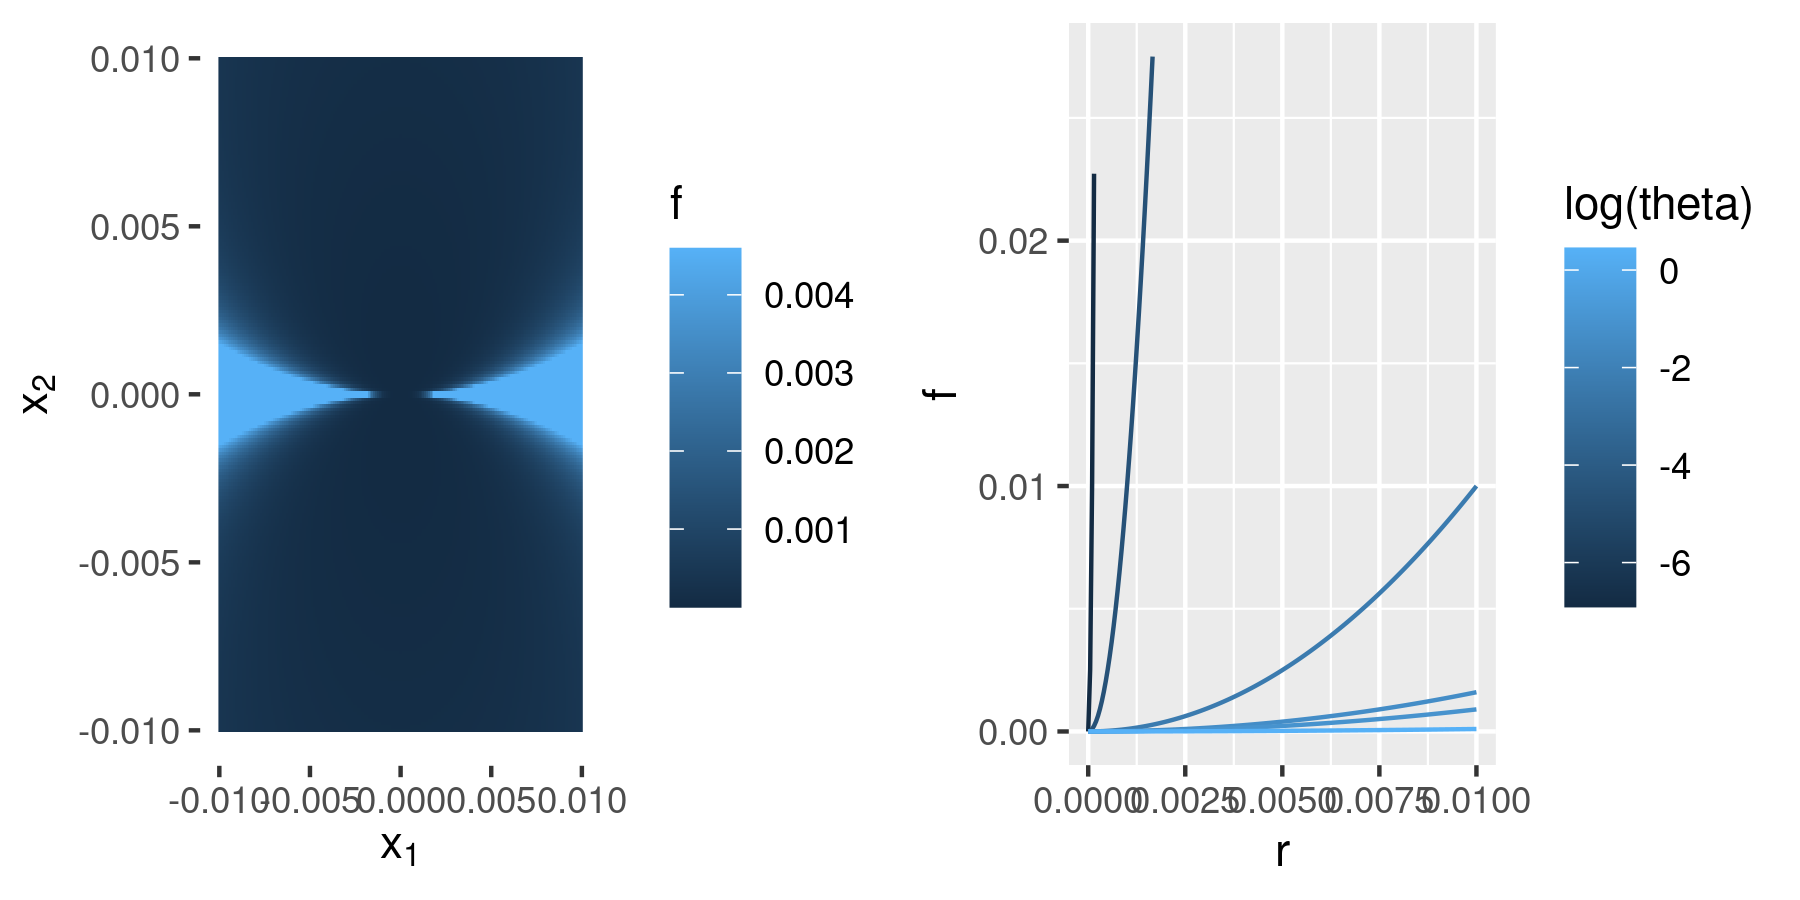
\includegraphics[width=0.980\linewidth,height=0.490\linewidth]{static_images/pathological_r2_example.png}
% \caption{A plot of $f(x_1, x_2)$ from \exref{r2_pathological}.}
% \figlabel{r2_pathological}
% \centering
% \end{figure}
%%%%%%%%%%%%%%%%%%%%%%%%%%%%%%%%%%%%%%%%%%%%%%%%%%%%%%%%%%%%%%%%%%%%%%%%%
%
\Figref{r2_pathological} contains a plot of $f(r, \theta)$, both over
$\mathbb{R}^2$ and along paths for particular choices of $\theta$.

We now show that $f$ has a directional derivative in every direction, but is not
Fr{\'e}chet differentiable.  By ordinary calculus, for any $\theta$,
$\fracat{\partial f(r, \theta)}{\partial r}{r=0} = 0$, so the directional
derivatives all exist and are identically $0$.  However, for any $r$, there
exists a $\theta(r)$ such that $r / |\sin(\theta(r))| = 1$.  For such a choice
of $\theta(r)$, the error in the linear approximation is $f(r, \theta(r)) - 0 =
1/2$, which does not go to zero as $r \rightarrow 0$.

\end{ex}
%%%%%%%%%%%%%%%%%%%%%%%%%%%%%%%%%%%%%%%%%%%%%%%%%%%%%%%%%%%%%%%%%%%%%%%%%

Fr{\'e}chet differentiability is only concerned with an infinitesimal
neighborhood.  The function can behave arbitrarily badly in a region just
outside the point at which the derivative is computed and retain Fr{\'e}chet
differentiability. In this sense, Fr{\'e}chet differentiability is a desirable
but not sufficient requirement if we are interested in extrapolating using
linear approximations.  The next example illustrates this fact.

%%%%%%%%%%%%%%%%%%%%%%%%%%%%%%%%%%%%%%%%%%%%%%%%%%%%%%%%%%%%%%%%%%%%%%%%%
%%%%%%%%%%%%%%%%%%%%%%%%%%%%%%%%%%%%%%%%%%%%%%%%%%%%%%%%%%%%%%%%%%%%%%%%%
\begin{ex}\exlabel{r2_pathological_v2}
%
In \exref{r2_pathological} second derivative in a particular direction is given
by $\fracat{\partial^2 f(r, \theta)}{\partial r^2}{r=0} = \frac{1}{2 |\sin
\theta|}$, which can be made arbitrarily large by taking $\theta$ close to $0$
or to $\pi$.  We could modify $f(r, \theta)$ to be Fr{\'e}chet differentiable by
smoothly ``capping'' $1 / |\sin \theta|$ at some arbitrarily large value.
However, the ability to meaningfully extrapolate $f(r, \theta)$ in the direction
of a very large but finite second derivative remains limited.

In the context of \exref{r2_pathological}, fix some $0 < M < \infty$,
and define
%
\begin{align*}
%
\tilde{f}(r, \theta) := \begin{cases}
    f(r, \theta) & \textrm{when }\frac{1}{\abs{\sin(\theta)}} \le M \\
    0. & \textrm{when }\frac{1}{\abs{\sin(\theta)}} > M.
%
\end{cases}
%
\end{align*}
%
Then $\tilde{f}$ is continuous and Fr{\'e}chet differentiable at $r=0$. In this
case, for any $r$, $\sup_{\theta} r / |\sin(\theta(r))| = r / M$, so  both
$\lim_{r \rightarrow 0} \tilde{f}(r, \theta) \le \lim_{r \rightarrow 0} r^2 /
M^2 = 0$ and $\lim_{r \rightarrow 0} \tilde{f}(r, \theta) / r \le \lim_{r
\rightarrow 0}  r / M^2 = 0$.  (Note that $\tilde{f}$ is continuous only
at $r=0$, not on a ball centered at $0$.)

Despite being Fr{\'e}chet differentiable, the linear approximation may not
extrapolate well to any finite $r$.  In the direction $\theta = \sin^{-1}(1 /
M)$, the error of the linear extrapolation to any $r_0$ is still $\tilde{f}(r,
\theta) - 0 = M r_0^2$. Since Fr{\'e}chet differentiability requires only $M <
\infty$, the extraplation error can be arbitrarily large, even for Fr{\'e}chet
differentiable functions.

\end{ex}
%%%%%%%%%%%%%%%%%%%%%%%%%%%%%%%%%%%%%%%%%%%%%%%%%%%%%%%%%%%%%%%%%%%%%%%%%

Given that \exref{r2_pathological} is neither Fr{\'e}chet differentiable nor
continuous, whereas \exref{r2_pathological} is both Fr{\'e}chet differentiable
and continuous, one might wonder whether Fr{\'e}chet differentiability is
equivalent to continuity.  In general, Fr{\'e}chet differentiability is stronger
than continuity, in the sense that Fr{\'e}chet differentiability implies
continuity, but continuity does not imply Fr{\'e}chet differentiability
\citep[Proposition 4.8 (d)]{zeidler:2013:functional}.  See also \citet[Example
1.9]{averbukh:1967:theory} for a simple example of a function on $\mathbb{R}^2$
that is continuous and directionally differentiable but not Fr{\'e}chet
differentiable.

The sort of pathology exhibited by \exref{r2_pathological, r2_pathological_v2}
requires some care to construct in $\mathbb{R}^2$, but requires some care to
avoid in infinite-dimensional spaces.  We now give an illustrative example in
the $\lp{p}$ spaces, which is closely related to the difficulties we encounter
analyzing $\KL{\eta, \phi}$ for $p \in [1, \infty)$.

%%%%%%%%%%%%%%%%%%%%%%%%%%%%%%%%%%%%%%%%%%%%%%%%%%%%%%%%%%%%%%%%%%%%%%%%%
%%%%%%%%%%%%%%%%%%%%%%%%%%%%%%%%%%%%%%%%%%%%%%%%%%%%%%%%%%%%%%%%%%%%%%%%%
\begin{ex}\exlabel{e_log_disocontinuous_v2}
%
Let us try to smooth the example \exref{e_log_disocontinuous_v1} by excising its
behavior on the pathological arguments that are unbounded below. Define
%
\begin{align*}
%
\tilde{f}(\gamma) = \begin{cases}
    f(\gamma) & \textrm{when }\inf_\theta \gamma(\theta) > -\infty \\
    0 & \textrm{otherwise}.
\end{cases}
%
\end{align*}

Note that if $\gamma$ satisfies $\inf_\theta \gamma(\theta) = -\infty$,
%
\begin{align*}
%
\tilde{f}(\t \gamma) = 0 \mathtxt{for any }\t > 0 \mathtxt{and} f(\phiz) = 0.
%
\end{align*}
%
So the discontinuity of \exref{e_log_disocontinuous_v1} no longer applies.
However, we will show that $\tilde{f}$ remains discontinuous in an $\lp{\mu,p}$
space under some mild conditions. Assume that $\mu \ll \lambda$, and that for a
given measure $\gamma \in \lp{\p,p}$ with $1 \le p < \infty$ and  $\p \ll \q$.

By continuity of the dominating Lebesgue measure (\lemref{continuity_partition})
there exists a positive sequence $\epsilon_n \rightarrow 0$, such that for each
$\epsilon_n$ there exists a set $S_n$ with $\p(S_n) = \epsilon_n$.
Since $\p \ll \q$, $\q(S_{\epsilon_n}) > 0$ as well.

For each $\epsilon_n$, and for a given $\c_n > 0$ and $0 < \delta_n < 1$, define
%
\begin{align*}
%
\gamma_n(\theta) :=
(\delta_n - 1)\ind{\theta \in S_{\epsilon_n}} +
\c_n \ind{\theta \notin S_{\epsilon_n}}.
%
\end{align*}
%
Then $\gamma_n(\theta) \in \lp{\p,p}$ with
%
\begin{align*}
%
\norm{\gamma_n}_{\p,p} ={}&
\norm{(\delta_n - 1) \ind{\theta \in S_{\epsilon_n}} +
      \c_n \ind{\theta \notin S_{\epsilon_n}}}_{\p,p}
\\\le{}&
    \abs{\delta_n - 1} \epsilon_n^{1/p} +
    \c_n ( 1 - \epsilon_n)^{1/p}
\mathand\\
%
\abs{\tilde{f}(\gamma_n) - \tilde{f}(\phiz)}
={}&
% \abs{
%     \q(S_\epsilon) \log(\delta) +
%     (1 - \q(S_\epsilon)) \log(1 + \c)
% }
% \\={}&
    \q(\epsilon_n) \abs{\log(\delta_n)} +
    (1 - \q(S_{\epsilon_n})) \log(1 + \c_n)
\\\ge{}&
    \q(S_{\epsilon_n}) \abs{\log(\delta_n)}.
%
\end{align*}
%,
Take $\delta_n = \exp(-1 / \q(S_{\epsilon_n}))$ and let $\c_n$ converge to a
finite constant.  Then, for all $n$, $\q(S_{\epsilon_n}) \abs{\log(\delta_n)}
= \q(S_{\epsilon_n}) / \q(S_{\epsilon_n}) = 1$, so
%
\begin{align*}
%
\abs{\tilde{f}(\gamma_n) - \tilde{f}(\phiz)} \ge{} 1
\mathtxt{and}
\norm{\gamma_n}_p \rightarrow{} 0.
%
\end{align*}
%
So $\tilde{f}$ is discontinuous at $\phiz$ in $\norm{\cdot}_{\p, p}$.
%
\end{ex}
%%%%%%%%%%%%%%%%%%%%%%%%%%%%%%%%%%%%%%%%%%%%%%%%%%%%%%%%%%%%%%%%%%%%%%%%%

Indeed, \exref{e_log_disocontinuous_v2} shows that the KL divergence cannot be
Fr{\'e}chet differentiable for $p < \infty$, even if it could somehow be safely
extended to functions outside $\pertset$.

%%%%%%%%%%%%%%%%%%%%%%%%%%%%%%%%%%%%%%%%%%%%%%%%%%%%%%%%%%%%%%%%%%%%%%%%%
%%%%%%%%%%%%%%%%%%%%%%%%%%%%%%%%%%%%%%%%%%%%%%%%%%%%%%%%%%%%%%%%%%%%%%%%%
%
\begin{thm}\thmlabel{kl_discontinuous}
%
Fix the quantities in \defref{prior_nl_pert} with $p \in [1, \infty)$.  Let
$\etaopt$ denote a VB optimum, and that $\KL{\q(\theta \vert \etaopt) ||
\pbase(\theta)}$ is well-defined. Then the map $\phi \mapsto \KL{\etaopt, \phi}$
is discontinuous at $\phiz$ on the set $\pertset$, in the sense that, for any
$\epsilon$, there exists a $\phi \in \pertset$ such that
%
\begin{align*}
%
\norm{\phi}_{\mu,p} \le \epsilon \mathand
\abs{\KL{\etaopt, \phiz} - \KL{\etaopt, \phiz}} \ge 1.
%
\end{align*}
%
Consequently, any version $\KLhat{\eta, \phi}$ of the KL divergence that
coincides with $\KL{\eta, \phi}$ on $\pertset$ is not, in general, Fr{\'e}chet
differentiable at $\etaopt, \phiz$.
%
\begin{proof}
%
% By continuity of the dominating Lebesgue measure
% (\lemref{continuity_partition}), there exists a sequence $\epsilon_n \rightarrow
% 0$ and sets $S_n$ such that $\pbase(S_{\epsilon_n}) = \epsilon_n$.
% $\KL{\q(\theta \vert \etaopt) || \pbase(\theta)}$ is well-defined, $\q(\theta
% \vert \etaopt)$ and $\pbase(\theta)$ are mutually absolutely continuous, so
% $\q(S_{\epsilon_n}) > 0$.

By \eqref{nl_vb_pert_p}, the KL divergence $\KL{\etaopt, \phi}$ is of the form
%
\begin{align*}
%
\KL{\etaopt, \phi} = \KL{\etaopt, \phiz} +
\expect{\q(\theta \vert \etaopt)}{
    \log\left(1 + \frac{\phi(\theta)}{p \pbase(\theta)^{1/p}}\right)
}.
%
\end{align*}
%
Let us choose a $\phi \in \pertset$.  Take $\beta = p$ and
%
\begin{align*}
%
\palt(\theta) ={}&
    \pbase(\theta)\left(
        \left( \frac{1 - \epsilon\delta}{1 - \epsilon}\right)^{p}
        \ind{\theta \notin S_{\epsilon}} +
        \delta^{p} \ind{\theta \in S_{\epsilon}}
    \right) \textrm{ so that}
\\
\phi(\theta) ={}& p \palt(\theta)^{1/p} - p \pbase(\theta)^{1/p}.
%
\end{align*}
%
So $\phi \in \pertset$.  Define $\gamma(\theta) = \phi(\theta) /
p \pbase(\theta)^{1/p}$, and note that $\gamma \in \lp{\pbase, p}$ with
$\norm{\gamma}_{\pbase, p} = \norm{\phi}_{\lambda, p}$, and
%
\begin{align*}
%
\KL{\etaopt, \phi} = \KL{\etaopt, \phiz} +
\expect{\q(\theta \vert \etaopt)}{\log\left(1 + \gamma(\theta)\right)}.
%
\end{align*}
%
The result then follows from \exref{e_log_disocontinuous_v2}, with $\p =
\pbase$,  $\q = \q(\theta \vert \etaopt)$, and $\c_n = (1 - \epsilon_n \delta_n) /
(1 - \epsilon_n)$.
%
\end{proof}
%
\end{thm}
%%%%%%%%%%%%%%%%%%%%%%%%%%%%%%%%%%%%%%%%%%%%%%%%%%%%%%%%%%%%%%%%%%%%%%%%%

Combinging \thmref{lp_derivative} and \thmref{kl_discontinuous}, we see that the
case of $p \in [1, \infty)$ is quite similar to \exref{r2_pathological}. Though
every directional derivative exists, the quality of the linear approximation can
be arbitrarily poor; in the $\lp{\mu,p}$ space, the role of $\theta$ near
integer multiples of $\pi$ is played by prior perturbations with density near
zero in small sets of nonzero measure.  To carry the analogy futher, one might
be tempted to further restrict $\phi$ so that $\p(\theta \vert \phi)$ is bounded
away from zero.  Even if it were possible to do so smoothly,
\exref{r2_pathological_v2} provides a cautionary warning.

Indeed, the tension between differentiability and expressiveness appears
fundamental.  Consider \figref{func_dist}.  These two densities are far from one
another according to KL divergence (from blue to red) since the red density has
nearly zero mass where the blue does not.  They are also distant from one
another in $\norminf{\cdot}$, since it takes a large multiplicative change to
turn a nonzero number into a nearly zero number.  However, the two densities are
close in $\norm{\cdot}_{p}$, since the region where the red density is nearly
zero has a small measure. In order for VB approximations to be continuous (a
necessary condition for Fr{\'e}chet differentiability), one must consider a
topology on priors that is no coarser than the topology induced by KL
divergence.  But since valid priors can take values close to zero, a sacrifice
in expressiveness of the neighborhood of zero must be made in order to induce a
topology that works with KL divergence.  Multiplicative changes and the
$\norminf{\cdot}$ norm make such a tradeoff in a natural, easy-to-understand
way.  If one desires a more expressive prior space, it seems to the authors more
fruitful to investigate variational divergences other than KL rather than
attempt to adapt the space of prior perturbations.

\FunctionDistFig{}

In light of the strong result of \thmref{eta_phi_deriv} and the negative result
of \thmref{kl_discontinuous}, we consider only $p = \infty$ and multiplicative
perturbations for our real-world experiments.
